%!TEX root = ../dissertation.tex
%\begin{savequote}[75mm]
%\qauthor{Quoteauthor Lastname}
%\end{savequote}

%% Set up problem
\begin{figure*}[t]
\begin{center}
{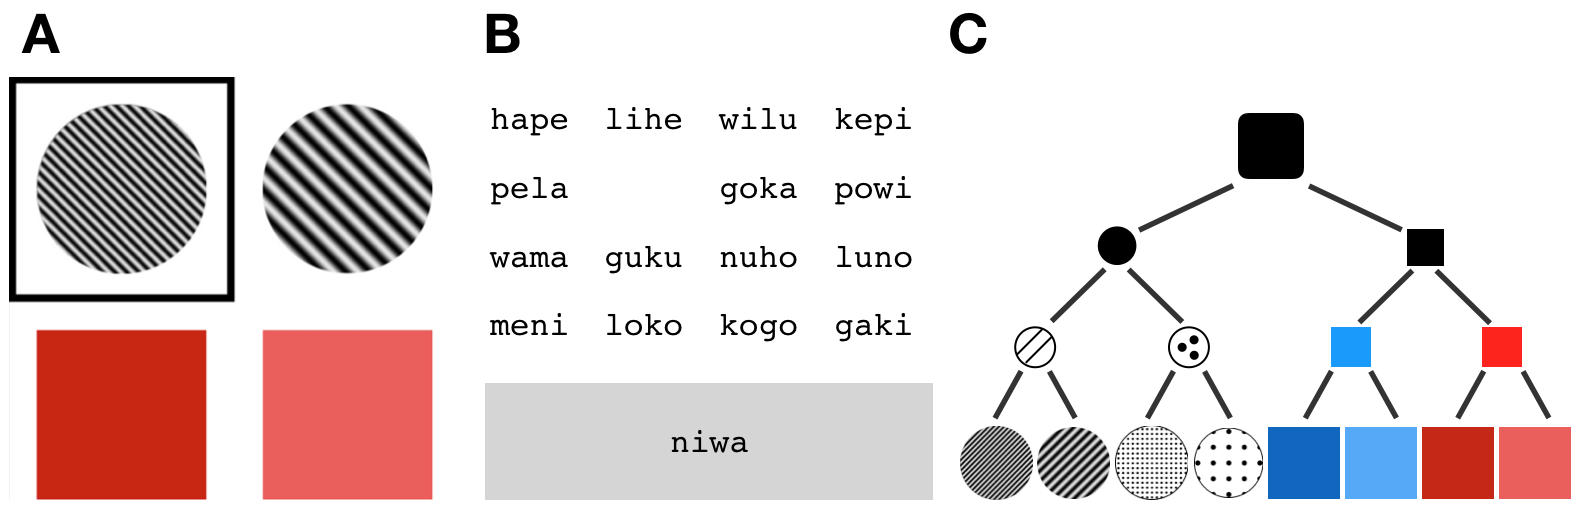
\includegraphics[scale=.63]{./figures/Sec2-design.png}}
{\caption{{(A) Example of \emph{fine} context where one of the distractors belongs to the same fine-grained branch of the hierarchy as the target (i.e.\ another striped circle), so any abstract label would be insufficient to disambiguate them. The target is highlighted for the speaker with a black square. (B) Drag-and-drop chat box interface. (C) Hierarchical organization of stimuli.\label{fig:context_design}}}}
\vspace{-2ex}
\end{center}
\end{figure*}

In the previous section, we examined a mechanism for rapid, partner-specific learning that allows agents to form stable but arbitrary \emph{ad hoc} conventions. 
While a degree of arbitrariness is central to conventionality -- there must exist more than one solution that would work equally well -- this does not necessarily imply that all possible conventions for a meaning are equally likely in practice, or even that all meanings are equally likely to become conventionalized in the first place \cite{HawkinsGoldstone16_SocialConventions}.

For example, while most English speakers have the basic-level word ``tree'' in their lexicon, along with a handful of subordinate-level words like ``maple'' or ``fir,'' we typically do not have labels exclusively referring to each individual tree in our yard.
If we need to refer to a specific tree, we instead create a referring expression \emph{on the fly.}
Meanwhile, we \emph{do} often have conventionalized labels (i.e. proper nouns) for individual people and places that we regularly encounter in our daily lives.
Why do conventions form at some levels of abstraction rather than others?
Here, we show how our proposed theory accounts for these key patterns of \emph{context-sensitivity} as arising naturally from communicative need in dyadic interaction.

In particular, functional accounts of linguistic conventions have frequently observed that lexical systems are well-calibrated to the statistics of the environment \cite{gibson2019efficiency}.
This ``optimal expressivity'' hypothesis has accounted well for the lexical distributions found in natural languages across semantic domains like color words and kinship categories \cite{KempRegier12_KinshipCategories,regier201511,gibson2017color,kemp2018semantic}, as well as the compositional systems that emerge under iterated learning with communication in the lab \cite{WintersKirbySmith14_LanguagesAdapt, KirbyTamarizCornishSmith15_CompressionCommunication}. 
For example, languages in warm regions ought to be more likely to collapse the distinction between ice and snow into a single word, simply because there are fewer occasions that require distinguishing between the two \cite{regier2016languages}. 

Thus, while there is abundant evidence for context-sensitivity in the \emph{outcomes} that result from convention formation processes, it is currently unclear what cognitive mechanisms are necessary to give rise to such outcomes.
That is, context-sensitivity has not yet been grounded in a cognitive and mechanistic account of the processes unfolding in the minds of individual agents as they interact.
Our inferential account hypothesizes that local context shapes the conventionalization process through the mechanisms of pragmatic reasoning over the shorter timescales of dyadic interactions.
%While our hypothesis about ad hoc conventionalization specifically concerned the shorter timescales of dyadic interaction, similar pressures may operate over the multi-generational timescales of cultural evolution. %,  operate on the shorter timescales of dyadic interaction. 
%Better understanding the effect of context on local conventions rapidly formed by adaptive agents over extended interactions may therefore be valuable for understanding how \emph{languages} are globally shaped by communicative constraints.
%Recent computational approaches to language evolution have argued that the lexical conventions of languages balance simplicity, or learnability, with the communicative needs of their users over longer timescales. 
%% Hypothesis
%Under the logic of a local efficiency/informativity tradeoff, we make two predictions about the emergence of abstractions in dyads. 


First, we fill a gap in the empirical literature by collecting a new dataset of human interactions under different environmental statistics.
This experiment manipulates the context of distractors in a repeated reference game where participants must interactively coordinate on an artificial language from scratch. %\cite<e.g.>{GalantucciGarrod11_ExperimentalSemiotics}.
% which allows us to examine the conventions that form in different communicative contexts.
Second, we compare different model predictions by reporting simulations of artificial agents interacting in the same contexts.
In both the empirical data and simulations, we find that conventions come to reflect the distinctions that are functionally relevant for communicative success. 
Furthermore, we find that pragmatic reasoning is necessary for these effects to arise. 
%% Example that sets up our specific hypothesis?

%Suppose, mixing thought experiments from \citeA{Wittgenstein09_PhilosophicalInvestigations} and \citeA{Quine13_WordAndObject}, that two travelers meet in a forest, with no language in common. One is cooking dinner, and the other agrees to help in exchange for food and shelter. What kind of micro-language do they coordinate on to solve this joint task, and how is it shaped by context? 
			
\subsection{Experimental methods}

\subsubsection{Participants}

We recruited 278 participants from Amazon Mechanical Turk to play an interactive, multi-player game using the framework described in \citeA{Hawkins15_RealTimeWebExperiments}. Pairs were randomly assigned to one of three different conditions, yielding approximately $n=37$ dyads per condition, after excluding participants who disconnected before completion.\footnote{Planned sample sizes, exclusion criteria, and behavioral analysis plan were pre-registered at \url{https://osf.io/2hkjc/}. We also ran an additional 53 participants in a third condition which we do not analyze here.}

\subsubsection{Procedure \& Stimuli}
Participants were paired over the web and placed in a shared environment containing an array of objects (Fig.\ \ref{fig:context_design}A) and a `chatbox' to send messages from a randomly generated vocabulary (Fig.\ \ref{fig:context_design}B). On each of 96 trials, one player (the `speaker') was privately shown a highlighted target object and allowed to send a single word to communicate the identity of this object to their partner (the `listener'), who subsequently made a selection from the array. Players were given full feedback, swapped roles each trial, and both received bonus payment for each correct response.

The objects that served as referents were designed to cluster in a fixed three-level hierarchy with shape at the top-most level, color/texture at the intermediate levels, and frequency/intensity at the finest levels (see Fig.\ \ref{fig:context_design}C). Each communicative context contained four objects. Distractors could differ from the target at various level of the hierarchy, creating different types of contexts defined by the finest distinction that had to be drawn. We focus on two: \emph{fine} trials, where the closest distractor belongs to the same fine-grained subordinate category (e.g.\ another striped circle; see Fig.\ \ref{fig:context_design}A), and \emph{coarse} trials, where the closest distractor belongs to a coarser level of the conceptual hierarchy (e.g.\ dotted circle instead of striped circle).\footnote{Even coarser trials with super-ordinate distractors (e.g.\ a circle target among three square distractors) were logically possible but would have introduced several experimental confounds; we opted to leave these trial types out of our design and conduct the minimal manipulation.} Fixed arrays of 16 utterances (enough to allow the potential for full expressibility) were randomly generated for each pair (and held constant across trials) by stringing together consonant-vowel pairs into pronounceable 2-syllable words (see Fig.\ \ref{fig:context_design}B).

Critically, we manipulated the statistics of the context in a between-subjects design to test the context-sensitivity of conventions. 
In the \emph{fine} condition, all targets appeared in fine contexts; in the \emph{course} condition, all targets appeared in course contexts; and in the \emph{mixed} condition, half of the targets appeared in each context.
Sequences of trials were constructed by randomly shuffling targets and trial types within blocks and ensuring no target appeared more than once in a row. 
In addition to behavioral responses collected over the course of the game, we designed a post-test to explicitly probe players' final lexica. For all sixteen words, we asked players to select all objects that a word can refer to (if any), and for each object, we asked players to select all words that can refer to it (if any). 
This bidirectional measure allows us to check the internal validity of the lexica reported.

\begin{figure}[t]
\begin{center}
{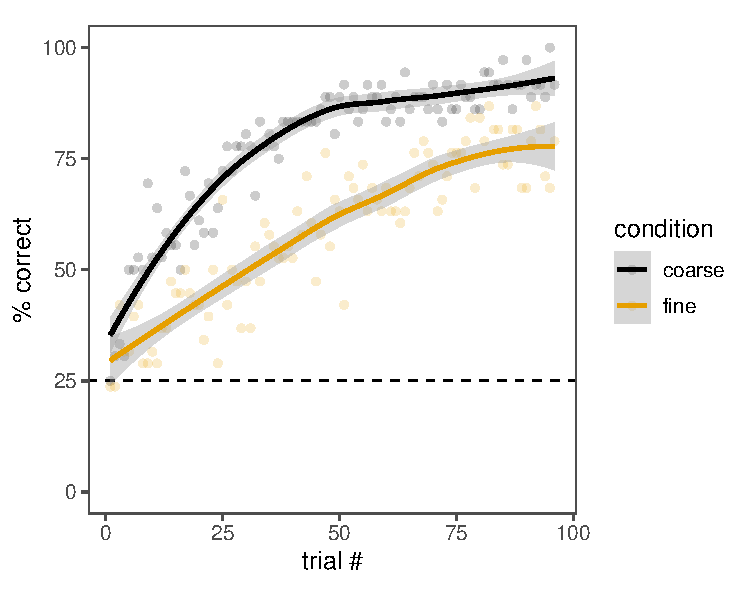
\includegraphics[scale=1]{./figures/sec2_empirical_accuracy.pdf}}
{\caption{{Players learn to coordinate on a successful communication system, but converge faster in the coarse condition than the fine condition. Each point is the mean proportion of correct responses by listeners; curves are nonparametric fits. 
\label{fig:context_accuracy}}}}
\vspace{-3ex}
\end{center}
\end{figure}

\subsection{Behavioral results}

\subsubsection{Partners successfully learn to communicate}

Although participants in all conditions began with no common basis for label meanings, performing near chance on the first trial (proportion correct $= 0.19$, 95\%~CI~$=~[0.13, 0.27]$), most pairs were nonetheless able to coordinate on a successful communication system over repeated interaction (see Fig.\ \ref{fig:context_accuracy}). 
A mixed-effects logistic regression on listener responses with trial number as a fixed effect, and including by-pair random slopes and intercepts, showed a significant improvement in accuracy overall, $z = 14.4, p < 0.001$. 
Accuracy also differed significantly \emph{across} conditions (Fig.\ \ref{fig:context_accuracy}): adding an additional main effect of condition to our logistic model provided a significantly better fit, $\chi^2(2) = 10.8, p = 0.004$. 
Qualitatively, the \emph{coarse} condition was easiest for participants, the \emph{fine} condition was hardest, and the \emph{mixed} condition was in between.
Finally, the (log) response time taken by the speaker to choose an utterance also decreased significantly over the course of the game, $t = -19.7, p < 0.001$, indicating that lexical mappings became increasingly established or accessible.



\begin{figure*}[t]
\begin{center}
\includegraphics[scale=0.75]{Sec2-results.pdf}
\caption{Pragmatic demands of context shape the formation of abstractions. (A) Mean number of words participants reported with specific meanings (applying to 1 object) or abstract meanings (applying to 2 objects). (B) Number of unique words used by speakers in each repetition block. (C)  Diversity of terms within reported lexica: many participants in the \emph{coarse} condition reported a mixture of abstract and specific terms. }
\label{fig:lexiconContent}
\end{center}
\end{figure*}


\subsubsection{Partners converge on similar conventions}

Another indicator of successful learning is convergence or alignment of lexica between partners within a dyad. 
Before using post-test responses to compute similarity between partners, however, we examine the internal consistency of an individual's post-test responses. 
For each participant, we counted the number of mismatches between the two directions of the lexicon question (e.g.\ if they clicked the word `mawa' when we showed them one of the blue squares, but failed to click that same blue square when we showed `mawa'). 
In general, participants were quite consistent: out of 128 cells in the lexicon matrix (16 words $\times$ 8 objects), the median number of mismatches was 2 (98\% agreement), though the distribution has a long tail (mean $= 7.3$). 
We therefore conservatively take a participant's final lexicon to be the \emph{intersection} of their word-to-object and object-to-word responses.

Using these estimates of each participant's lexicon, we compute the overlap between partners. 
For most pairs, partners aligned strongly by the end, with a median post-test overlap of 97.6\% (125 out of 128 entries). 
Because these matrices were extremely sparse, however, just a a few mismatches could have a large impact on performance. 
Overall accuracy in the game is strongly correlated with alignment: partners who reported more similar lexica at the end tended to perform significantly better at the task ($r = 0.77$).  

Despite these markers of success at the group level, individual performance was bimodal: a subpopulation of 29 games (11\% of coarse games, 18\% of mixed, and 39\% of fine) still showed relatively poor performance, sometimes near chance, by the end of the game. 
For the subsequent analyses focusing on the content of the lexicon, we exclude games with fourth-quartile accuracy below the pre-registered criterion of 75\% to ensure we are examining only successful lexica. 

\subsubsection{Contextual pressures shape the lexicon}

We predicted that in contexts regularly requiring speakers to make fine distinctions among objects at subordinate levels of the hierarchy, we would find lexicalization of specific terms for each object (indeed, a one-to-one mapping may be the most obvious solution in a task with only 8 objects). Conversely, when no such distinctions were required, we expected participants to adaptively lexicalize more abstract terms. One coarse signature of this prediction lies in the \emph{efficiency} of the resulting lexicon: lexicalizing abstract terms should require participants to use fewer terms overall.

To test this prediction, we counted the number of words in each participant's reported lexicon (i.e.\ the words for which they marked at least one object in the post-test). We found that participants in the \emph{coarse} condition reported significantly smaller, more efficient lexica ($m = 4.9$ words) than participants in the \emph{fine} condition ($m = 7.6, t = 9.5, p < 0.001$; see Fig.\ \ref{fig:lexiconContent}A). At the same time, the smaller lexicon provided equivalent coverage of objects: the median number of objects where participants agreed on the same word was 7 in both conditions. 

How did these lexica emerge over the course of interaction? 
To measure the effective vocabulary size used throughout the interaction, we considered the total number of unique words produced within each repetition block.
Because all eight objects appeared as the target once in each block, this measure takes a maximum value of 8, in the case where a different word was used for every object, and a minimum value of 1, in the case where the same word was used for every object.
We constructed a mixed-effects regression model predicting the effective vocabulary size, including fixed effects of condition and repetition block, and random intercepts and effects of repetition block for each dyad. 
We found an overall main effect of condition, with participants in the fine condition using significantly fewer words across all repetition blocks ($m = 4.9$ in coarse, $m=6.8$ in fine, $t = 9.5, p < 0.001$).
However, we also found a significant interaction: the effective vocabulary size gradually increased over time in the fine condition but remained roughly constant in the coarse condition, $b = 0.06, t = 4.5, p < 0.001$, see Fig. \ref{fig:lexiconContent}B.
This interaction is consistent with gradual differentiation based on communicative need in the fine condition.

Finally, if participants in the \emph{coarse} condition could get away with fewer words in their lexicon, what are the meanings of the words they do have? 
We counted the numbers of `specific' terms (e.g.\ words that refer to only one object) and `abstract' terms (e.g.\ words that refer to two objects) in the post-test. 
We found that the likelihood of lexicalizing abstractions differed systematically across conditions (see Fig.\ \ref{fig:lexiconContent}A). 
Participants in the \emph{fine} condition reported lexica containing exclusively specific terms, while participants in the \emph{coarse} condition reported significantly more abstract terms ($m = 2.5, p < 0.001$). 
The modal system in the fine condition was exactly eight specific terms with no abstract terms, and the modal system in the coarse condition was exactly four abstract terms (red, blue, striped, spotted) with no specific terms.
However, these data also reveal an interesting asymmetry in lexicon content across conditions: while abstractions are nearly absent from the \emph{fine} condition, individual participants in the course condition often reported a mixture of terms at differently levels roughly following a Pareto frontier (see Fig.\ \ref{fig:lexiconContent}C).

\subsection{Model simulations}

Our empirical results show that different communicative contexts systematically lead to different communicative conventions.
Critically, the sequence of targets was held constant across conditions; only the distractors were manipulated.
This task poses several distinct challenges for models of coordination and convention formation.
First, the context constantly changes, with a subset of only four of the eight total objects shown on each trial.
Second, the stimuli are embedded in a conceptual taxonomy, where some objects are more similar than others.
In this section, we show how our model explains such sensitivity as the consequence of pragmatic reasoning \cite<e.g.>{GoodmanFrank16_RSATiCS,FrankeJager16_ProbabilisticPragmatics} over a space of taxonomic word meanings.

We evaluate the extent to which local context shapes our agents' conventions through a series of simulations.
For each dyad in our human dataset, we pair up two artificial agents and present them the same stimulus sequence of targets and contexts that human participants saw.
Our artificial agents swapped speaker and listener roles on each trial, as human participants did, and updated their beliefs after each trial using their own history: that is, while we matched the stimulus sequence, the models did not observe human data. 

Following \citeA{XuTenenbaum07_WordLearningBayesian}, we consider a space of meanings that reflects the conceptual structure of the stimulus hierarchy. 
In addition to 8 meanings at the sub-ordinate level (one for each individual object), we populate the hypothesis space with 4 meanings at the basic-level (striped, spotted, blue, red), 2 meanings at the super-ordinate level (circle and square), 1 exhaustive meaning (shape), and 1 ``null'' meaning, which does not apply to any of the objects.
We populate the utterance space with 8 single-word labels, which simplifies the speaker model: the utterance cost term is constant across all utterances, so it does not have an effect on speaker behavior.
Finally, we note that the simplicity prior over the lexicon space penalizes meanings with larger extensions, so \emph{a priori}, agents have an inductive bias toward subordinate terms.
For ease of presentation, we consider the parameter setting of $\alpha_L=5,\alpha_S=10$ and memory discounting parameter of $\beta = 0.8$ (see Model comparison below for a more thorough evaluation of these parameters).

\begin{figure}[t]
\begin{center}
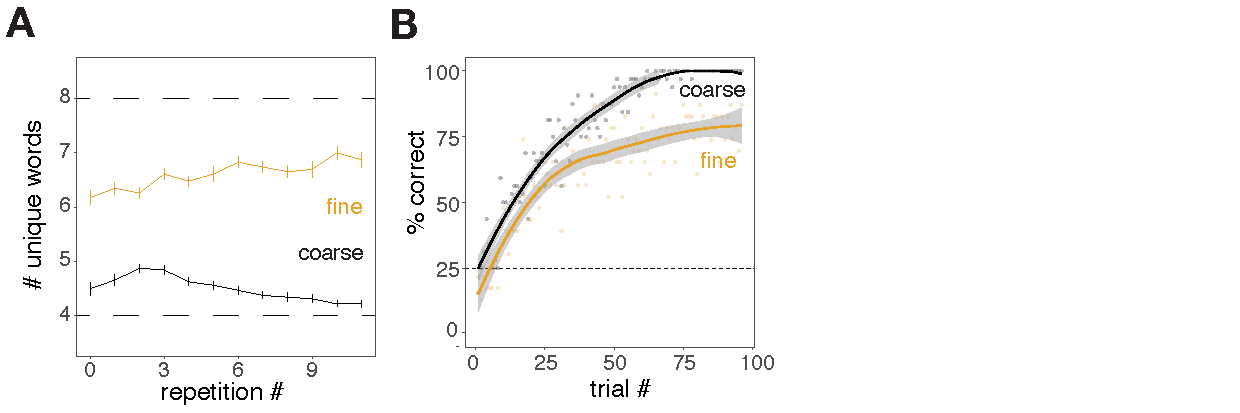
\includegraphics[scale=0.6]{./figures/sec2-modelFig.pdf}
\vspace{-1ex}
{\caption{{Model simulations. (A) Speakers gradually use a larger lexicon size across conditions, and (B) coordinate more quickly in the coarse condition than the fine condition, as observed in the empirical data.}  \label{fig:sec2model}}}
\end{center}
\vspace{-3ex}
\end{figure}


\paragraph{Simulation 2.1: Context-sensitivity}

First, we compare the model's learning curves across context conditions (Fig. \ref{fig:sec2model}B). 
We focus on the \emph{coarse} and \emph{fine} conditions for simplicity, since this single comparison captures the core phenomena of interest.
In a mixed-effects logic regression, we find that communicative accuracy steadily improves over time across conditions, $b=0.72, z = 16.9, p<0.001$.
However, we also find a significant interaction with condition: the rate of improvement is significantly higher in the coarse condition than the fine condition, $b=-0.49, z=9.3, p <0.001$. 
These effects track our qualitative findings in the human data: our artificial agents are able to successfully coordinate, but do so more easily in the coarse condition than the fine condition. 

Second, we examine the effective vocabulary sizes that emerge from our simulations. 
We use the same measure of unique words produced in each repetition block that we used in our analyses of human data above. 
In an identical mixed-effects model, we again an overall main effect of condition, with participants in the fine condition using significantly fewer words across all repetition blocks ($m = 4.7$ in coarse, $m=6.5$ in fine, $t = 4.5, p < 0.001$).
However, we also found a significant interaction: the effective vocabulary size gradually increased over time in the fine condition compared to the coarse condition, $b = 0.18, t = 8.1, p < 0.001$, see Fig. \ref{fig:sec2model}A.
These effects suggest that the model converges to roughly the same lexicon sizes as humans do.

Finally, we examine more closely the emergence of terms at different levels of abstraction.
We have access not only to the outward behavior of our simulated agents, but also their internal \emph{beliefs} about their partner's lexicon.
So we can not only query these beliefs at the very \emph{end} of the game, as we did in our empirical post-test, we can also directly examine the evolution of these beliefs from the very beginning of the interaction.
At each time point in each game, we take the single meaning with highest probability for each word.

In Fig. \ref{fig:evolution}, we show the proportion of words with meanings at each level of abstraction, collapsing across all games in each condition.
Most critically for comparison with empirical data, we find that the \emph{final} proportion of basic-level vs. subordinate-level terms is significantly different across the coarse and fine conditions.
Only 9\% of words had subordinate-level meanings (green) in the coarse condition, compared with 79\% in the fine condition, $\chi^2(1) = 436, p < 0.001$.
At the same time, 45\% of words had basic-level meanings (blue) in the coarse condition, compared with only 8\% in the fine condition, $\chi^2(1) = 136, p < 0.001$.
The remaining words in each condition were assigned the `null` meaning (red), consistent with an overall smaller effective vocabulary size in the coarse condition.
These effects are consistent with human post-test responses.

What dynamics give rise to these final proportions?
Qualitatively, we observe that agents begin with assumptions of `null' meanings due to their simplicity prior but quickly begin assigning meanings based on their partner's usage.
In both conditions, both basic-level meanings and simpler subordinate-meanings are consistent with the data, with a general preference for simpler meanings.
After the first repetition block, however, agents in the coarse condition begin pruning out some of the subordinate-level terms and become increasingly confident of basic-level meanings and agents in the fine condition become even more confident of subordinate level meanings. 

\begin{figure}[t]
\begin{center}
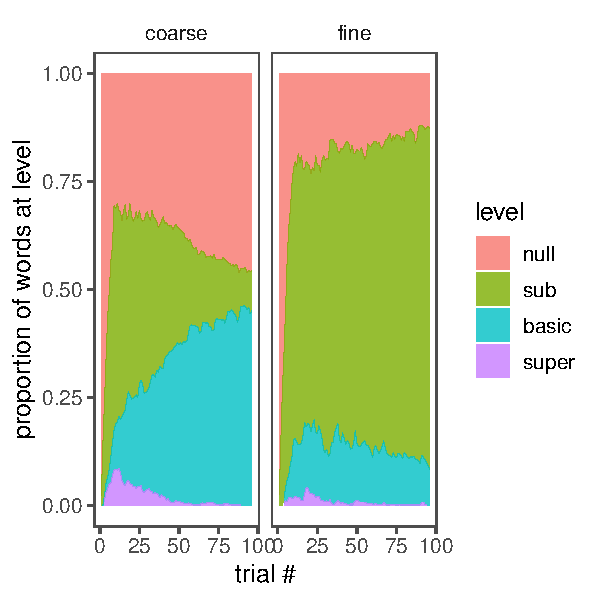
\includegraphics[scale=0.75]{evolution.pdf}
\caption{Proportion of terms at different levels of abstraction in different conditions }
\label{fig:evolution}
\end{center}
\end{figure}


\paragraph{Model comparison}

\rdh{TODO: we need to decide which comparisons are most interesting. may need to implement baseline model from other papers (e.g. Steels-style, or Spike et al. implementation?) for a more explicit comparison to models outside our class of Bayesian agents...}

We compare our model to (1) a simpler case when both agents condition on the same data (i.e. the true target) even after an unsuccessful communication attempt, and (2) ask what happens when we manipulate forgetting parameter, or remove it?

In a non-pragmatic variant of our model, agents use words proportional to their literal meaning and assume their partner is doing the same. 
In this case, their lexicon converges to a degenerate 1-word (shape) state.
Because an initial usage is consistent with all levels of abstraction, one of the agents will eventually extend the same word to different object. 
Then the only way to subsequently accommodate this extension in the interaction history is to rule out more specific meanings. 
The non-pragmatic agent has no way of knowing that this degenerate solution is confusing to their partner, and will continue to prefer it because it's literally true of every object.

\subsection{Discussion}

How does context shape conventions? 
There is abundant evidence that languages adapt to the needs of their users, and the context-sensitive emergence of abstractions demonstrated in this section suggests that the driver of this adaptation may lie in the rapid adaptability of agents in individual dyadic interaction. 
By manipulating context statistics in a real-time experiment, we evaluated the extent to which our model captured patterns of context-sensitivity in the behavioral data.

Previous proposals have handled context-sensitivity in different ways.
In some common settings for convention formation, there is no explicit representation of context at all, as in the task known as the ``Naming Game'' where agents coordinate on names for objects in isolation \cite{steels2012experiments,baronchelli2008depth}. 
In other common settings, context is central but held constant throughout interactions, as in Lewis signaling games \cite{lewis_convention:_1969}, where agents use a fixed set of messages to communicate a fixed set of world states \cite{skyrms2010signals,BrunerEtAl14_LewisConventions}.

One of the most sophisticated studies of context in prior work is the Discrimination Game of \citeA{steels2005coordinating}, which examined the joint formation of color categories and color naming conventions.
As in our experiments, contexts were generated randomly on each trial from a large space and stimuli are embedded in a similarity space (with similarity based on Euclidean distance in continuous space rather than taxonomic relations).
Unlike our task, contexts were not systematically manipulated, and the resulting level of abstraction was not evaluated: the only restriction was to ensure that color chips were a fixed minimum distance apart  \cite<see also>[which found that imposing a realistic Just Noticeable Difference function as the minimum distance on communicative contexts leads to human-like color naming systems]{baronchelli2010modeling}.

In models using Roth-Erev reinforcement learning update rules or simple neural networks, the referential context is sometimes accounted for with a \emph{lateral inhibition} heuristic used by both the speaker and listener agents \cite{franke2012bidirectional}.
If communication is successful, the connection strength between the label and object is not only increased, the connection between the label and competing objects (and, similarly, between the object and competing labels) is explicitly \emph{decreased} by a corresponding amount \cite<see also>{steels2005coordinating}.
This lateral inhibition heuristic is functionally similar to our pragmatic reasoning mechanism, in terms of allowing the agent to learn from negative evidence (i.e. the speaker's choice \emph{not} to use a word, or the listener's choice \emph{not} to pick an object). 
Under an inferential framework, however, this property emerges as a natural consequence of well-established Gricean principles of pragmatic reasoning.
Reasoning about a partner's intentions, either while updating beliefs about their lexicon or while selecting an action, naturally instantiates a kind of inductive bias for \emph{mutual exclusivity} \cite{gulordava2020one,ohmerreinforcement,FrankGoodmanTenenbaum09_Wurwur}.

Our results may help to illuminate the relationship between our concepts and words, which are often treated interchangeably. While our mental taxonomies are adaptive to the natural perceptual structure of the world \cite{MervisRosch81_CategorizationReview} %(Rosch et al, 1976; Mervis \& Rosch ,1981; Murphy \& Smith, 1982), 
it is far from inevitable that all levels of these conceptual hierarchies become conventionalized as lexical items. There are many perfectly natural concepts that are not represented by distinct words in the English language: for instance, we do not have words for each tree in our yards, or for ad-hoc concepts %like \emph{things to sell at a garage sale} 
\cite{Barsalou83_AdHocCategories}. Indeed, English speakers are often fascinated by foreign words like the Danish ``hygge'' (a specific notion of coziness) or Scottish ``tartle'' (hesitating when introducing someone because you've forgotten their name) that are difficult to express in English.
Our results highlight communicative needs to distinguish, in context, as a force behind the choice to lexicalize some fine-grained concepts. 
A related direction for future work is to explore the relationship between communicative need and \emph{basic-level} structure.

While we showed how abstract words emerge from efficiency even in a task requiring only reference to individual objects, there are other clear functional advantages to having abstract terms in the lexicon. For one, they allow speakers to efficiently refer to large, potentially infinite, sets of things, and make generalizations about categories, e.g.\ ``Dogs bark'' \cite{TesslerGoodman16_Generics}. Future work should explore this as an additional pressure toward abstract, nested nouns.
Similarly, the option to refer to more specific concepts with compound terms (e.g.~``spotted dog''), which was not available in our experiment, may impact final conventions.
We expect that labels will become lexicalized when the cost incurred by frequently using a compositional construction exceeds the cost of adding an additional word to the lexicon. 
Future work should also explore these hypotheses about how lexicalization of nominal terms trades off with compositionality. 
Our shared lexical conventions are richly structured systems with meanings at multiple levels of abstraction. 
We are constantly supplementing our existing language with local conventions, as we need them.
